% Created by tikzDevice version 0.12.3 on 2019-11-08 10:06:16
% !TEX encoding = UTF-8 Unicode
%\documentclass[10pt]{article}
%\usepackage{tikz}
%
%\usepackage[active,tightpage,psfixbb]{preview}
%
%\PreviewEnvironment{pgfpicture}
%
%\setlength\PreviewBorder{0pt}
%
%\usepackage{amsfonts}
%\usepackage{bm}\begin{document}

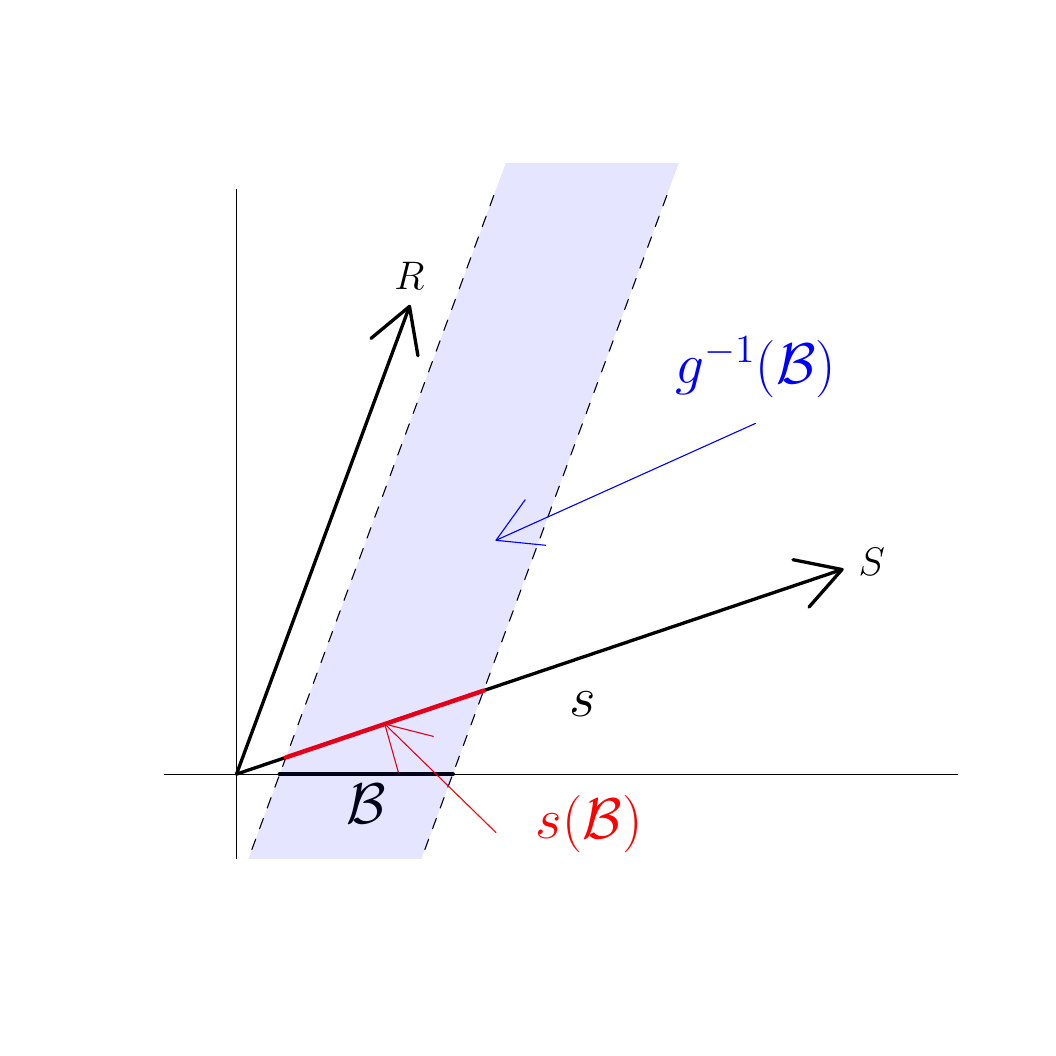
\begin{tikzpicture}[x=1pt,y=1pt]
\definecolor{fillColor}{RGB}{255,255,255}
\path[use as bounding box,fill=fillColor,fill opacity=0.00] (0,0) rectangle (361.35,361.35);
\begin{scope}
\path[clip] ( 49.20, 61.20) rectangle (336.15,312.15);
\definecolor{drawColor}{RGB}{0,0,0}

\path[draw=drawColor,line width= 0.4pt,line join=round,line cap=round] ( 75.46, 49.37) --
	( 75.46,302.86);

\path[draw=drawColor,line width= 0.4pt,line join=round,line cap=round] ( 12.94, 91.62) --
	(361.35, 91.62);

\path[draw=drawColor,line width= 1.2pt,line join=round,line cap=round] ( 75.46, 91.62) -- (294.26,165.55);

\path[draw=drawColor,line width= 1.2pt,line join=round,line cap=round] (282.33,151.98) --
	(294.26,165.55) --
	(276.55,169.10);

\node[text=drawColor,anchor=base west,inner sep=0pt, outer sep=0pt, scale=  1.00] at (300.26,163.26) {{\Large ${\bm S}$}};

\node[text=drawColor,anchor=base,inner sep=0pt, outer sep=0pt, scale=  1.00] at (200.49,112.53) {{\huge $\mathfrak{s}$}};

\path[draw=drawColor,line width= 1.2pt,line join=round,line cap=round] ( 75.46, 91.62) -- (137.97,260.61);

\path[draw=drawColor,line width= 1.2pt,line join=round,line cap=round] (141.02,242.80) --
	(137.97,260.61) --
	(124.07,249.07);

\node[text=drawColor,anchor=base,inner sep=0pt, outer sep=0pt, scale=  1.00] at (137.97,266.61) {{\Large ${\bm R}$}};

\path[draw=drawColor,line width= 0.4pt,dash pattern=on 4pt off 4pt ,line join=round,line cap=round] ( 75.46, 49.37) --
	(169.23,302.86);

\path[draw=drawColor,line width= 0.4pt,dash pattern=on 4pt off 4pt ,line join=round,line cap=round] (137.97, 49.37) --
	(231.75,302.86);

\path[draw=drawColor,line width= 1.6pt,line join=round,line cap=round] ( 91.09, 91.62) --
	(153.60, 91.62);

\node[text=drawColor,anchor=base,inner sep=0pt, outer sep=0pt, scale=  1.00] at (122.34, 73.88) {{\huge $\mathcal{B}$}};
\definecolor{drawColor}{RGB}{255,0,0}

\path[draw=drawColor,line width= 1.6pt,line join=round,line cap=round] ( 93.32, 97.65) --
	(164.77,121.79);
\definecolor{drawColor}{RGB}{0,0,0}

\node[text=drawColor,anchor=base west,inner sep=0pt, outer sep=0pt, scale=  1.00] at (183.63, 68.20) {{\huge $\color{red}{s(\mathcal{B})}$}};
\definecolor{drawColor}{RGB}{255,0,0}

\path[draw=drawColor,line width= 0.4pt,line join=round,line cap=round] (169.23, 70.49) -- (129.04,109.72);

\path[draw=drawColor,line width= 0.4pt,line join=round,line cap=round] (146.55,105.26) --
	(129.04,109.72) --
	(133.93, 92.33);
\definecolor{fillColor}{RGB}{0,0,255}

\path[fill=fillColor,fill opacity=0.10] ( 59.83,  7.12) --
	(122.34,  7.12) --
	(247.38,345.10) --
	(184.86,345.10) --
	cycle;
\definecolor{drawColor}{RGB}{0,0,255}

\node[text=drawColor,anchor=base,inner sep=0pt, outer sep=0pt, scale=  1.00] at (263.01,232.76) {{\huge $\color{blue}{g^{-1}(\mathcal{B}})$}};

\path[draw=drawColor,line width= 0.4pt,line join=round,line cap=round] (263.01,218.36) -- (169.23,176.11);

\path[draw=drawColor,line width= 0.4pt,line join=round,line cap=round] (179.79,190.78) --
	(169.23,176.11) --
	(187.21,174.30);
\end{scope}
\end{tikzpicture}
%\caption{a caption}
%\end{document}
